\documentclass[crop=false,10pt]{standalone}
\usepackage{standard}

\begin{document}
  \section{The Model} % (fold)
  \label{sec:The Model}
    \begin{figure*}[h]
      \center
      \begin{subfigure}[c]{0.49\textwidth}
        \center
        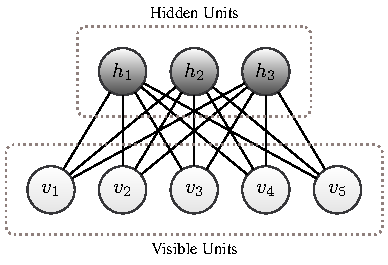
\includegraphics[scale=1.15]{figures/rbm-scheme-inputs.pdf}
      \end{subfigure}
      \begin{subfigure}[c]{0.49\textwidth}
        \center
        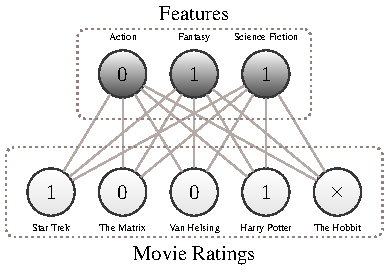
\includegraphics[scale=1.15]{figures/rbm-scheme-example.pdf}
      \end{subfigure}
      \caption{%
        The left part of the figure shows a schematic example of an RBM.
        The nodes are separated into visible and hidden units and connections are only allowed between those two subsets.
        The right part shows an example application to the collaborative filtering problem of predicting movie ratings.
        For one user the visible values are the movie ratings and the hidden values are some features, like movie genres, implicitly learned by the RBM.
      }
      \label{fig:rbm-scheme-and-example}
    \end{figure*}

    \subsection{Basic Idea} % (fold)
    \label{sub:basic_idea}
      To understand the model of an RBM let us first consider the basic idea by looking at the left part of figure \ref{fig:rbm-scheme-and-example}.
      It shows a simple schematic example of an RBM.
      At first sight there seems to be no real difference to a standard feed-forward neural network (FFNN) with two layers.
      But the subtle difference lies in the fact that every edge connecting different units in an RBM has to be undirected and not directed as in a typical FFNN.
      Therefore the influence of one unit to another cannot be computed directly through a feed-forward pass.
      \cite{Murphy2012}

      Apart from this there are two obvious properties which are defining the RBM.
      First, the units in the RBM are separated into two subsets, the hidden units and the visible units.
      Second, connections between units are only allowed between those two subsets.
      This makes it possible to equivalently define an RBM to be an undirected bipartite graph.
      \cite{Murphy2012,Montufar2018}

      These properties give us no real obvious interpretation for the values of these units.
      But we have to remember that we want to model a probability distribution over ratings.
      Based on this mathematically we will try to interpret every unit as a binary random variable.
      Later, this will enable us to sample from the probability distribution represented by the RBM and predicting the outcome.
      Interpreting user ratings to be realizations of the visible random variables we can then see that every visible value in an RBM stands for a movie rating made by some user.
      The realizations of the hidden random variables can be thought of as non-observable features the RBM has learned implicitly.
      \cite{Hinton2007,Murphy2012,Montufar2018}

      Looking at the right part of figure \ref{fig:rbm-scheme-and-example} one sees an example of these ideas for an imaginary user.
      Every rating from one user can be seen as a visible value.
      Based on these visible values an RBM can assign some hidden values based on some learned features, like movie genres \enquote{Action} or \enquote{Fantasy}.
      These hidden values for example would describe if the user likes the movie genre.
      \cite{towardsdatascience}

      Until now we have described how to model the collaborative filtering problem by an RBM but not how to model the RBM itself.
      Hence, we first have to define some parameters to be able to represent a set of probability distributions which can be learned.
      The procedure for an RBM is straightforward.
      We choose the standard approach of introducing biases for every unit and weights for every edge.
      Therefore we get two bias vectors for the hidden and visible units and one weight matrix for all connections.
      Figure \ref{fig:rbm-scheme} shows this schematically.
      \cite{Murphy2012,Hinton2007,Hinton2010,Montufar2018}
      \begin{figure}
        \center
        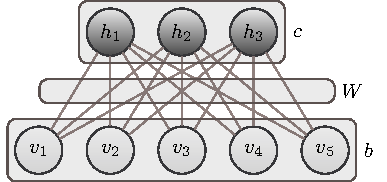
\includegraphics[width=0.441\textwidth]{figures/rbm-scheme.pdf}
        \caption{%
          The figure shows the basic scheme of an RBM with the weight matrix $W$ and bias vectors $b$ and $c$ as parameters describing the probability distribution modelled by the RBM.
        }
        \label{fig:rbm-scheme}
      \end{figure}
    % subsection basic_idea (end)

    \subsection{Mathematical Details} % (fold)
    \label{sub:mathematical_details}
      For the sake of simplicity, we will only assume so-called binary RBMs with binary hidden and visible values $\mathscr{B}\define\set{0,1}{}$ and will further on describe them only as RBMs.
      These RBMs are fundamental to every generalization and are not that much of a constraint.
      According to \cite{Hinton2007} and \cite{Murphy2012} binary RBMs can be easily extended to categorical RBMs or Gaussian RBMs.
      But it turns out that it is important for the hidden values to stay binary to introduce a sort of information bottleneck which strongly regularizes the mathematical properties of an RBM.
      \cite{Murphy2012,Hinton2007,Hinton2010,Montufar2018}

      \begin{definition*}[\small RBM]
        For $n,m\in\setNatural$ an RBM $ϑ$ is given by a tuple $(W,b,c)$ consisting of its weight matrix $W$, visible bias vector $b$ and hidden bias vector $c$.
        \[
          ϑ \define (W,b,c) \in \setReal^{(n\times m) + n + m}
        \]
        We call $n$ the number of visible units and $m$ the number of hidden units of ϑ.
      \end{definition*}

      As seen in figure \ref{fig:rbm-scheme} the mathematical definition of an RBM as data structure is straightforward.
      We want to keep such an approach for the parameterization of the probability distribution as well.
      Therefore we will first define the influence of every unit with respect to its connections by introducing an energy term.
      In this energy term every weight and bias linearly connects visible and hidden values.
      To model non-trivial probability distributions we need some simple non-linear function with good properties to be applied to this energy term.
      Afterwards, we have to make sure the resulting function is normalized such that it satisfies the definition of a probability distribution.
      \cite{Hinton2007,Hinton2010,Murphy2012}

      % To be precise, here and in the following we will assume $n\in\setNatural$ visible units and $m\in\setNatural$ hidden units for an RBM.
      % The sets $V$ and $H$ for all visible value vectors $v$ and hidden value vectors $h$ are then given by the following expressions.
      % \[
      %   v \in V \define \set{0,1}{}^n
      %   \separate
      %   h \in H \define \set{0,1}{}^m
      % \]

      % The parameters describing the RBM are taken to be real numbers.
      % We will abbreviate the weight matrix and the two bias vectors as one parameter.
      % This will make the following formulas much more readable.
      % \[
      %   ϑ \define (W,b,c) \in \setReal^{(n\times m) + n + m}
      % \]

      \begin{definition*}[\small RBM Probability Distribution]
        Let $n,m\in\setNatural$ and ϑ be an RBM with $n$ visible and $m$ hidden units.
        The probability distribution of ϑ is then given by $p[ϑ]$.
        \[
          \function{p[ϑ]}{\mathscr{B}^n\times \mathscr{B}^m}{[0,1]}
        \]
        \[
          p[ϑ](v,h) \define \frac{1}{Z(ϑ)} e^{ -E[ϑ](v,h) }
        \]
        Here, the energy term $E[ϑ](v,h)$ is given by the following expression.
        \[
          E[ϑ](v,h) \define -\transpose{v}Wh - \transpose{v}b - \transpose{h}c
        \]
        $Z(ϑ)$ is the normalization factor of $p[ϑ]$.
        \[
          Z(ϑ) \define \sum_{v\in \mathscr{B}^n} \sum_{h\in \mathscr{B}^m} e^{ -E[ϑ](v,h) }
        \]
      \end{definition*}

      % Now we will define the probability distribution the RBM is modelling with respect to its parameters.
      % This is a definition and not a corollary.
      % Of course, we could choose another approach.
      % But this would not be a RBM.
      % \[
      %   \function{p[ϑ]}{V\times H}{[0,1]}
      % \]
      % \[
      %   p[ϑ](v,h) \define \frac{e^{ -E[ϑ](v,h) }}{Z(ϑ)}
      % \]
      % Here we define $E[ϑ]$ to be the so called energy function of the RBM.
      % We have already introduced non-linearity by the exponential function.
      % Therefore one chooses $E[ϑ]$ as simple as possible.
      % \[
      %   \function{E[ϑ]}{V\times H}{\setReal}
      % \]
      % \[
      %   E[ϑ](v,h) \define -\transpose{v}Wh - \transpose{v}b - \transpose{h}c
      % \]
      % For completeness the normalization will be supplied.
      % The definition for $Z(ϑ)$ is straightforward and not important for the learning or inference processes.
      % \[
      %   Z(ϑ) \define \sum_{v\in V} \sum_{h\in H} e^{ -E[ϑ](v,h) }
      % \]

      At this point one could think, that we have introduced a major design problem in our RBM model.
      If we cannot observe hidden values then how should we be able to use a probability distribution with hidden values as its arguments.
      We can omit this problem by inserting a layer of indirection.
      We will simply use only the probability distribution for the visible values.
      For convenience here we use function overloading.
      \[
        \function{p[ϑ]}{\mathscr{B}^n}{[0,1]}
        \separate
        p[ϑ](v) \define \sum_{h\in \mathscr{B}^m} p[ϑ](v,h)
      \]
      This finishes the complete mathematical description of the RBM model.
      But because of the main properties of an RBM it seems appropriate to deduce a proposition for the posterior probability to show one big advantage of an RBM.
      Due to its property that connections are only allowed between hidden and visible values we know that under a given visible value vector the coordinates of the hidden value vector have to be independent and vice versa.
      So for all $v\in\mathscr{B}^n$ and $h\in\mathscr{B}^m$ one obtains the following.
      \cite{Hinton2010,Murphy2012}
      \[
        \begin{aligned}
          p[ϑ](h \vert v)
          &= \prod_{j=1}^m p[ϑ]\roundBrackets{h_j=1 \middle\vert v} \\
          &=\prod_{j=1}^m \sigm\roundBrackets{c_j + \sum_{i=1}^n v_i W_{ij}}
        \end{aligned}
      \]
      \[
        \begin{aligned}
          p[ϑ](v \vert h)
          &= \prod_{i=1}^n p[ϑ]\roundBrackets{v_i=1 \middle\vert h} \\
          &=\prod_{i=1}^n \sigm\roundBrackets{b_i + \sum_{j=1}^m W_{ij} h_j}
        \end{aligned}
      \]
      The logistic sigmoid function $\sigm$ is given by the typical definition.
      \[
        \function{\sigm}{\setReal}{(0,1)}
        \separate
        \sigm(x) \define \frac{1}{1+e^{-x}}
      \]
    % subsection mathematical_details (end)
  % section The Model (end)
\end{document}